% Table 1. use \table1{\textwidth}{caption 
% reference with \fullref{tab:table1}}
\def\table1#1#2{
\begin{tableminipage}{#1}
\customlabel{tab:table1}{\textbf{Table 1}}~{#2}\\[1em]
\begin{tabularx}{\textwidth}{@{}XXXX@{}}
\hline
{\bf Student} & {\bf Grade}\footnote{This is an example of a footnote in a table. Lowercase, superscript italic letters (a, b, c, etc.) are used by default. You can also use *, **, and *** to indicate conventional levels of statistical significance, explained below the table.} & {\bf Rank} & {\bf Notes} \\
\hline
John & 82\% & 1 & Performed very well.\\
Bob & 65\% & 3 & Not up to his usual standard.\\
Charlie & 73\% & 2 & A good attempt.\\
\hline
\end{tabularx}
\end{tableminipage}
}

% Figure 1. use \figure1{0.35}{caption}
% reference with \fullref{fig:figure1}}
\def\figure1#1#2#3{
\begin{minipage}{\textwidth}
    \customlabel{fig:figure1}{\textbf{Figure 1}} #2\\[1em]
    \twocolstart
    \fbox{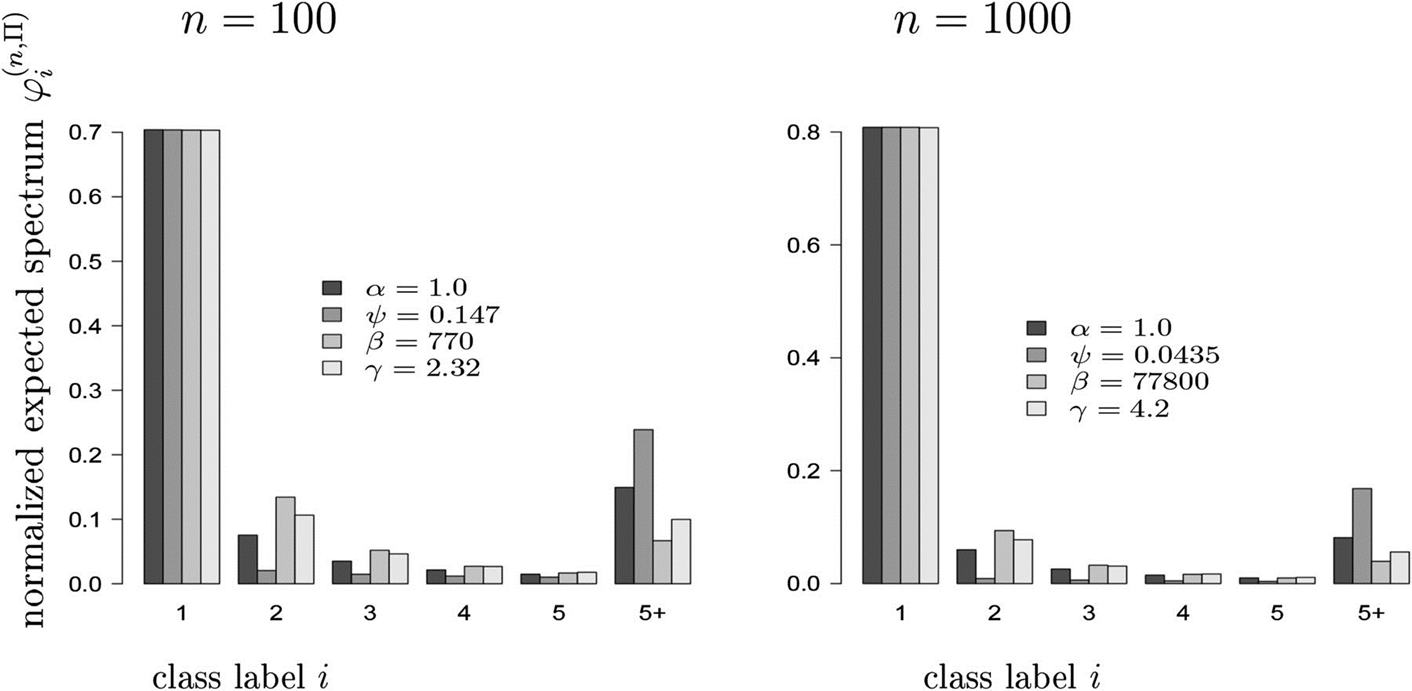
\includegraphics[scale=#1]{templates/example-figure.png}}
    \fbox{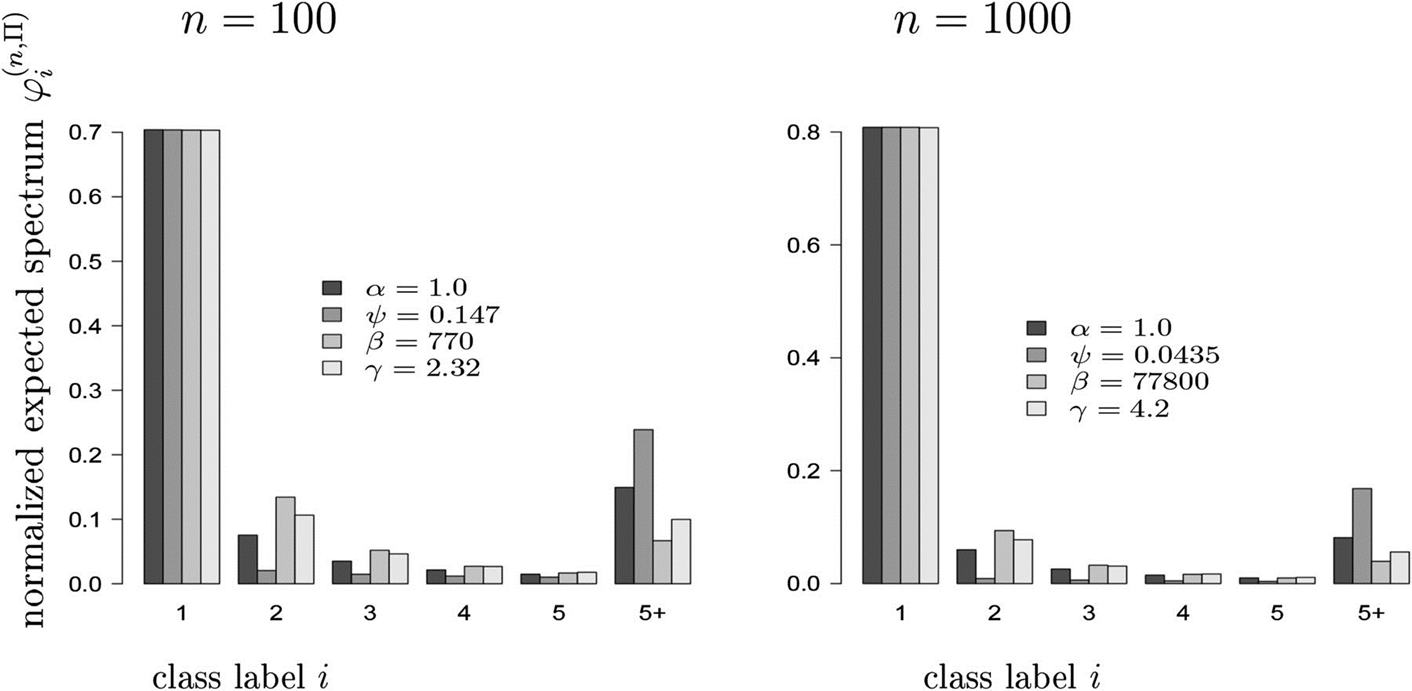
\includegraphics[scale=#1]{templates/example-figure.png}}
    \twocolend
    {\small #3}
\end{minipage}
}
%\def\figure1#1#2{
%\customlabel{fig:figure1}
%\framebox{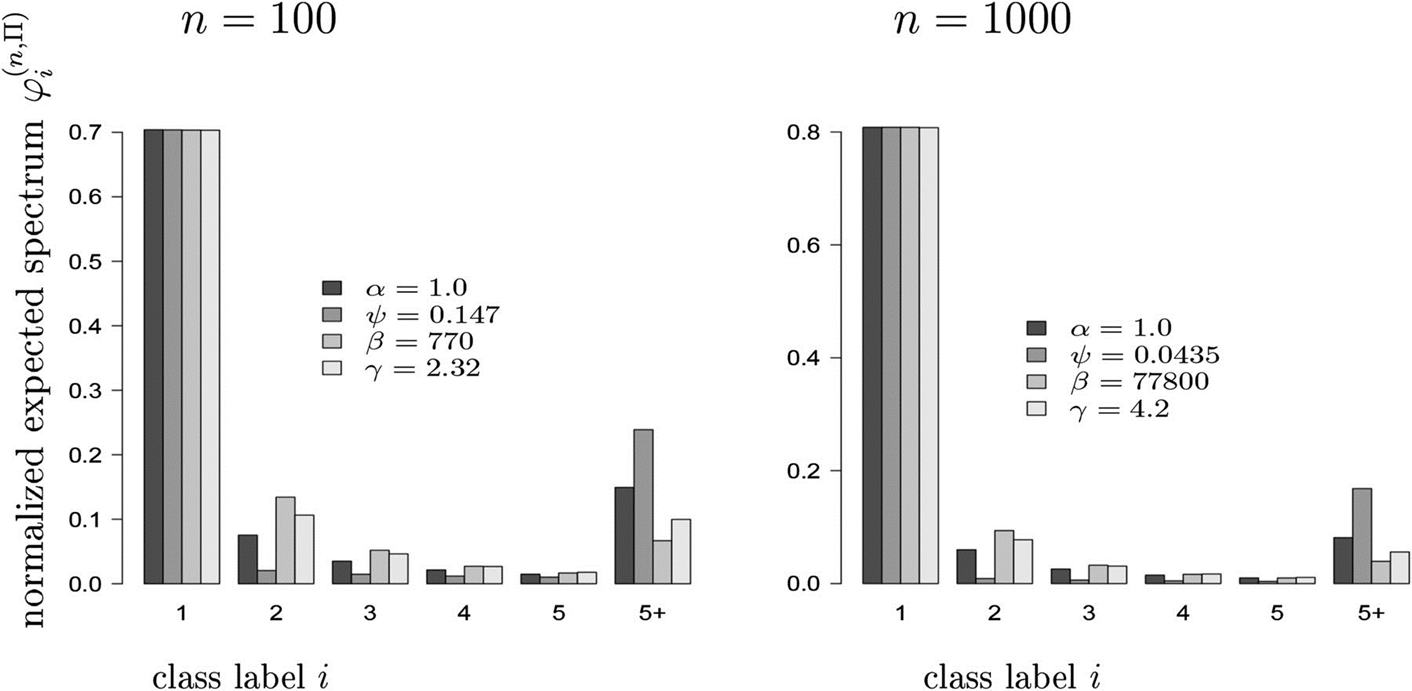
\includegraphics[scale = #1]{templates/example-figure.png}}\\[1em]
%\parbox[t]{0.5\textwidth}{\customlabel{fig:figure1}{\textbf{Figure 1}} #2}
%}

\endinput